\documentclass[a4paper,12pt]{jsbook}
\setlength{\textwidth}{\fullwidth}
\setlength{\evensidemargin}{\oddsidemargin}
\usepackage{thesis}
\usepackage{makeidx}
\usepackage{amsmath}
\usepackage{txfonts, float}
\usepackage{here}
\usepackage[dvipdfmx]{graphicx}
%\usepackage[noto-otc, unicode]{pxchfon}
\usepackage{listings,jvlisting}
\lstset{
  basicstyle={\ttfamily},
  identifierstyle={\small},
  commentstyle={\smallitshape},
  keywordstyle={\small\bfseries},
  ndkeywordstyle={\small},
  stringstyle={\small\ttfamily},
  frame={tb},
  breaklines=true,
  columns=[l]{fullflexible},
  numbers=left,
  xrightmargin=0zw,
  xleftmargin=3zw,
  numberstyle={\scriptsize},
  stepnumber=1,
  numbersep=1zw,
  lineskip=-0.5ex
}

\begin{document}

% 表紙
\thesis{卒業論文}
\date{2023年1月12日}
\title{
    \scalebox{1.5}{Y00-量子暗号における増幅の効果
}
}
\teacher{相馬 正宜 教授}
\organization{玉川大学 工学部 情報通信工学科}
\author{酒寄 遥}

\maketitle

% 前書き
%\chapter*{概要}
\thispagestyle{empty}

%\frontmatter
\tableofcontents
%\listoffigures
%\listoftables

% 本文
\mainmatter
%\chapter{How To Use \LaTeX}

\section{Figure}
    \subsection{基本的な画像挿入方法}
    写真はimg下に配置します.\\
    \begin{figure}[htbp]
        \centering   
        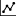
\includegraphics[width=0.5\textwidth]{img/sample/sample_png.png}
        \caption[sample image (png)]{sample image: when its extension is png.}
        \label{fig:sample_png}
    \end{figure}
    labelで指定することで, \figref{fig:sample_png}はxxxのように参照することができる.\\
    captionでは [] が目次に示される内容で, \{\} が本文に示される内容である. 同じでいい場合は \{\} のみで良い.\\
    上記のように, pngやjpegのようなラスタ画像を用いると, 拡大したときに荒くなってしまう.\\
    下記のようにpdfのようなベクタ画像を用いると拡大しても荒くならない.
    ただし, 保存時にベクタ形式にする必要がある.
    \begin{figure}[htbp]
        \centering   
        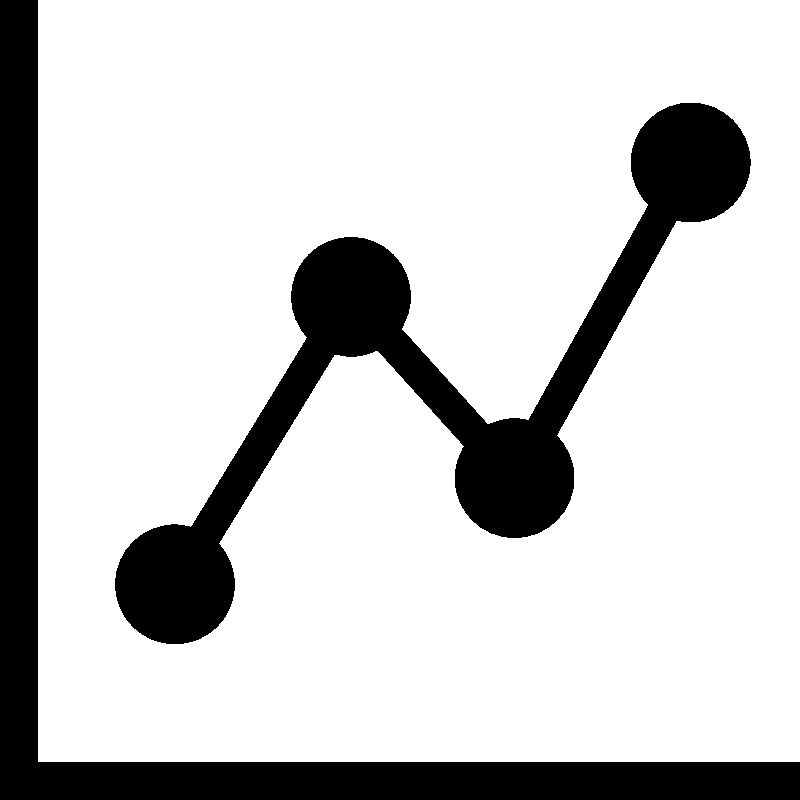
\includegraphics[width=0.5\textwidth]{img/sample/sample_pdf.pdf}
        \label{Fig:sample_pdf}
        \caption[sample image (pdf)]{sample image: when its extension is pdf.}
    \end{figure}
    出力の位置は[htbp]で指定するが, レイアウトによっては自動的に次のページに移動するなど, 指定した通りに配置できないときがある.\\
    この場合は[H]のように大文字で指定すると,
    \begin{figure}[H]
        \centering   
        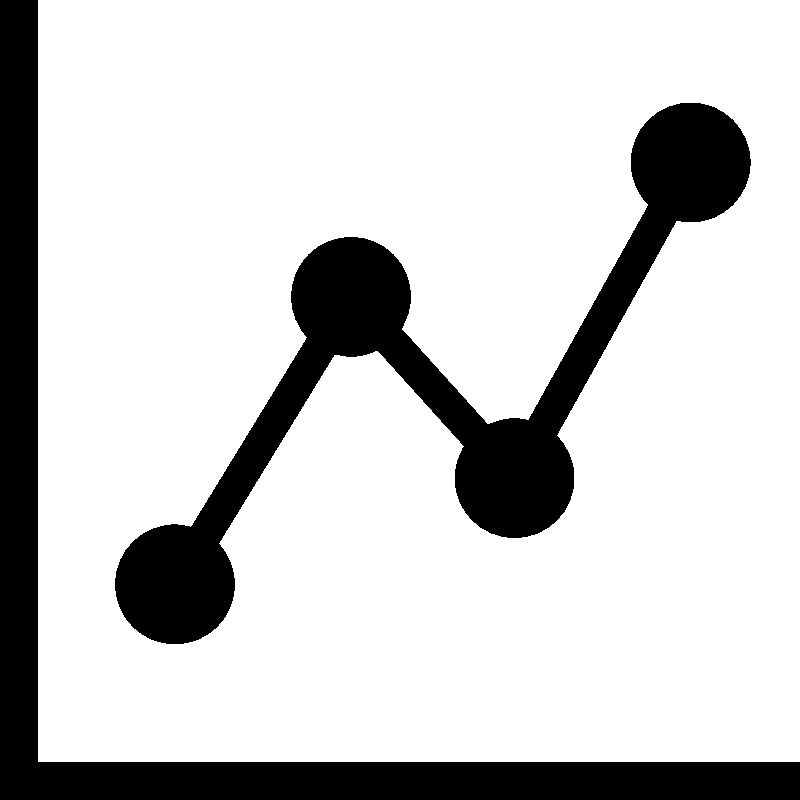
\includegraphics[width=0.5\textwidth]{img/sample/sample_pdf.pdf}
        \label{Fig:sample_pdf_here}
        \caption[sample image (pdf, here)]{sample image: when its extension is pdf and is enforced to be here.}
    \end{figure}
    このように強制的に配置が可能になる.

    \subsection{複数画像の挿入}
    複数画像の挿入方法はいくつかあるようだが, とりあえず下記で挿入することが可能.
    \begin{figure}[H]
		\centering
		\begin{tabular}{c}
		% ----- image 1 =====
			\begin{minipage}{0.25\hsize}
				\centering
				
\includegraphics[width=\textwidth]{img/sample/sample1.pdf}
				\text{(a)}
			\end{minipage}
		% ----- image 2 =====
			\begin{minipage}{0.25\hsize}
				\centering
				
\includegraphics[width=\textwidth]{img/sample/sample2.pdf}
				\text{(b)}
			\end{minipage}
		% ----- image 3 =====
			\begin{minipage}{0.25\hsize}
				\centering
				
\includegraphics[width=\textwidth]{img/sample/sample3.pdf}
				\text{(c)}
			\end{minipage}
		% ----- image 4 =====
			\begin{minipage}{0.25\hsize}
				\centering
				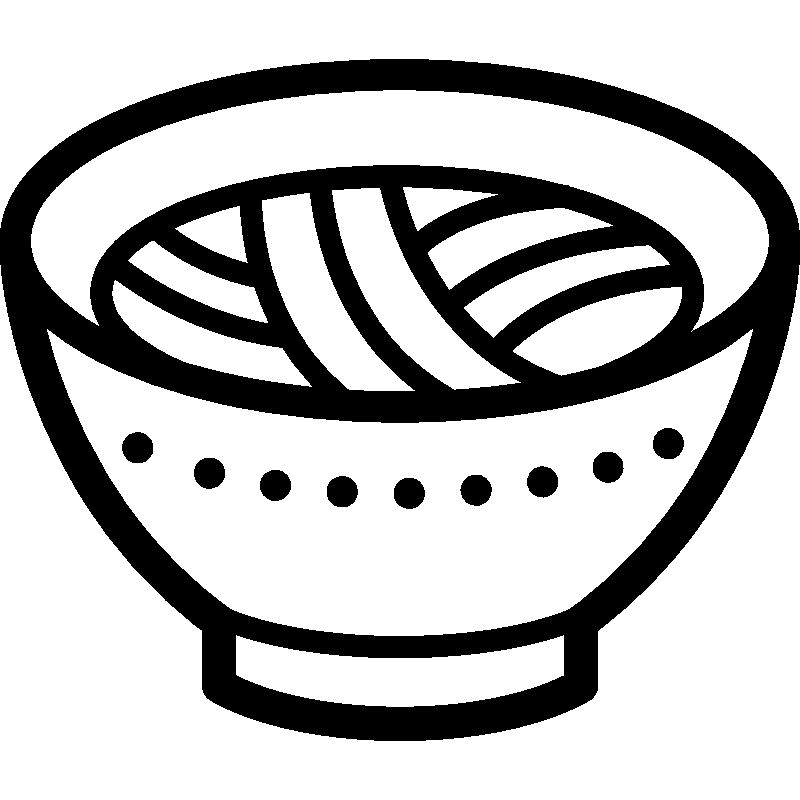
\includegraphics[width=\textwidth]{img/sample/sample4.pdf}
				\text{(d)}
			\end{minipage}
		\end{tabular}
		\caption[Four sample images]
		{
			Four sample images.
			(a) sushi (b) milk (c) peach (d) ramen
		}
		\label{fig:sample_four_images}
	\end{figure}

    縦2横2にすることも可能.
    \begin{figure}[H]
		\centering
		\begin{tabular}{c}
		% ----- image 1 =====
			\begin{minipage}{0.25\hsize}
				\centering
				
\includegraphics[width=\textwidth]{img/sample/sample1.pdf}
				\text{(a)}
			\end{minipage}
			\hspace{1cm}
		% ----- image 2 =====
			\begin{minipage}{0.25\hsize}
				\centering
				
\includegraphics[width=\textwidth]{img/sample/sample2.pdf}
				\text{(b)}
			\end{minipage}
			\vspace{1cm}\\
		% ----- image 3 =====
			\begin{minipage}{0.25\hsize}
				\centering
				
\includegraphics[width=\textwidth]{img/sample/sample3.pdf}
				\text{(c)}
			\end{minipage}
			\hspace{1cm}
		% ----- image 4 =====
			\begin{minipage}{0.25\hsize}
				\centering
				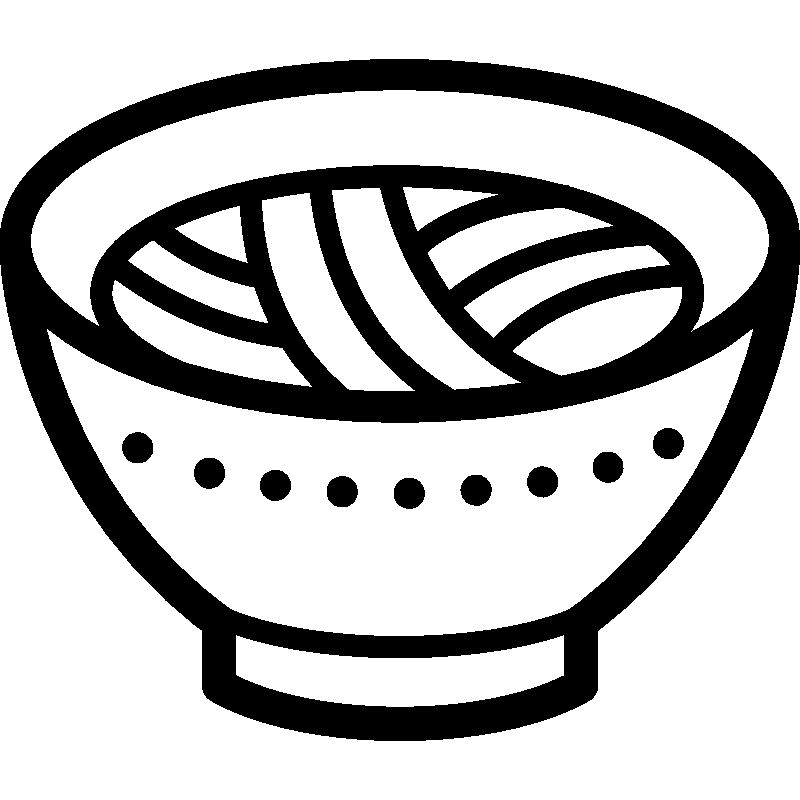
\includegraphics[width=\textwidth]{img/sample/sample4.pdf}
				\text{(d)}
			\end{minipage}
		\end{tabular}
		\caption[Four sample images]
		{
			Four sample images 2.
			(a) sushi (b) milk (c) peach (d) ramen
		}
		\label{fig:sample_four_images2}
	\end{figure}
    
\section{Table}
Tableは\tbref{tb:sample_table}のようにして挿入する.
\begin{table}[H]
	\centering
	\caption{Sample Table: accuracy for train/evaluation data.}
	\begin{tabular}{ll}\hline
		 訓練データの正答率&: $98\%$ \\
		 テストデータの正答率&: $88\%$ \\
	\label{tb:sample_table}
	\end{tabular}
\end{table}

\section{Bib}
参考文献は, \cite{author:06}とすれば良い.
複数の参考文献を扱う場合は, \cite{author:06, conference:06}のようにする.\\
使用してない参考文献は自動的に記載されないようになっているので, とりあえずbib/liter.bibに入れておいて構わない.\\
通し番号は本文で言及された順になるがこれも自動的に処理されるので気にしなくて良い.

\section{Equation}
数式の入力はたくさんある.
文章中であれば, $x = 2$ のように挿入できる.\\
数式環境を用意する場合は, \equref{eq:sample1}, \equref{eq:sample2}, \equref{eq:sample3}のようにできる.

\begin{align}
    x &= 2 \label{eq:sample1}\\
    y &= x^2 + 1 \label{eq:sample2}\\
      &= 5 \label{eq:sample3}
\end{align}


\begin{equation}\rho_0=(1−db)|vac\rangle\langle vac|+b
\sum_{k=1}^{d}|k\rangle\langle k| \label{sample_rho_0}
\end{equation}

\begin{equation}
\begin{split}
\rho_1&=(1−\eta)((1−db)|vac\rangle\langle vac|+bI)+\eta\rho\\
&=(1−\eta)(1−db)|vac\rangle\langle vac|+(1-\eta)bI+\eta\rho
\end{split} \label{sample_rho_1}
\end{equation}

\section{プログラム}
プログラムを掲載するには以下のようにする。

\begin{lstlisting}[caption=hoge,label=fuga]
# -*- coding: utf-8 -*-
import cmath
import math
import numpy
from scipy.stats import norm
import numpy as np
import numpy.linalg as LA
import matplotlib.pyplot as plt
\end{lstlisting}

\section{記号をそのまま出力}

\verb|abc_xy|
 % 使い方を示す例
\chapter{序論}

\section{本研究の目的と方法}
本論文では、Y00-量子暗号のシミュレーションシステムを用いて減衰通信路に対して、正規受信者の誤り率を評価する。そのとき、受信者側の最大信号強度の設定値を送信者側と一致させる場合と、受信者側の最大信号強度の設定値を減衰の効果を考慮して決める場合を比較する。


\section{本論文の構成}
本論文は本章を含め, 7つの章と2つの付録からなる.
\begin{itemize}
	\item 第1章では本論文の位置づけについて記した.
	\item 第2章では背景について記した.
	\item 第3章では提案手法について記した.
	\item 第4章では実験について記した.
	\item 第7章では提案手法に関して結論を考察し, 今後の展望に関して述べた.
	\item 付録Aではその他の本研究に関する予備実験や補足事項について述べた.
	\item 付録Bではその他の実験を載せた.
\end{itemize}
x\chapter{光の状態
}

コヒーレント状態$|\alpha\rangle$は、理想的なレーザー光を表している量子状態で、複素振幅$\alpha=x+iy$を持っている。また複素平面上で平均ベクトル$(x,y)^T$と共分散行列
$$
\begin{pmatrix}
1/4&0\\
0&1/4
\end{pmatrix}
$$
の正規分布に従って揺らいでいる。そしてコヒーレント状態を一般化したものが量子ガウス状態である。量子ガウス状態は、平均ベクトル$(x,y)^T$と共分散行列
$$
\begin{pmatrix}
a&c\\
c&b
\end{pmatrix}
$$
で表される。ただし共分散行列の要素は、関係式
$a+b\geq 0$,$ab-c^2\geq1/16$
を満たす必要がある。
スクイズド状態$|\alpha,\zeta\rangle$はガウス状態の一種で、図1のように量子揺らぎを持っている。スクイズド状態は、複素数$\alpha,\zeta$によって特徴づけられる。特に$\alpha$を$x+iy$,$\zeta$を$re^{i\theta}$とすると、
\begin{equation}
\begin{split}
a&=1/4[\cosh 2r-\sinh 2r\cos\theta]\\
b&=1/4[\cosh 2r+\sinh 2r\cos\theta]\\
c&=1/4\sinh 2r\sin\theta
\end{split}
\end{equation}
によって平均ベクトル$(x,y)^T$と共分散行列
\begin{equation}
\begin{pmatrix}
a&c\\
c&b
\end{pmatrix}
\end{equation}
が決まる。

\begin{figure}[htbp]
        \centering   
        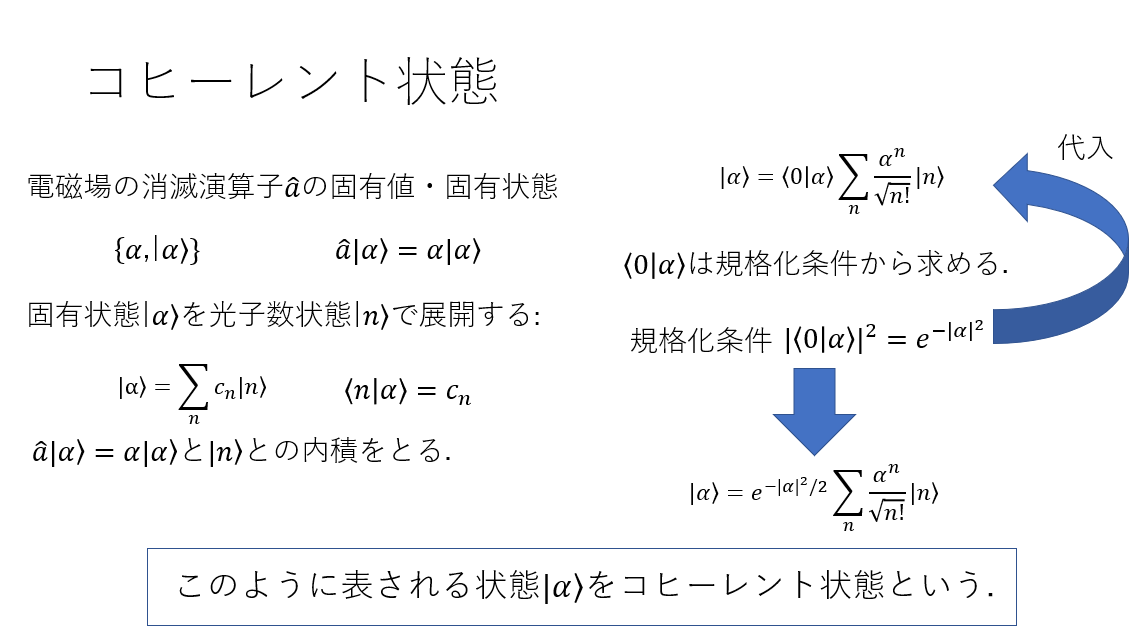
\includegraphics[width=1.0\textwidth]{img/zemi9.png}
        \caption[sample image (png)]{コヒーレント状態.}
        \label{Fig:1_5_1}
    \end{figure}
    
    \figref{Fig:1_5_1}はコヒーレント状態の定義を表している。コヒーレント状態は電磁場の消滅演算子の固有状態として与えられる。
    
\begin{figure}[htbp]
        \centering   
        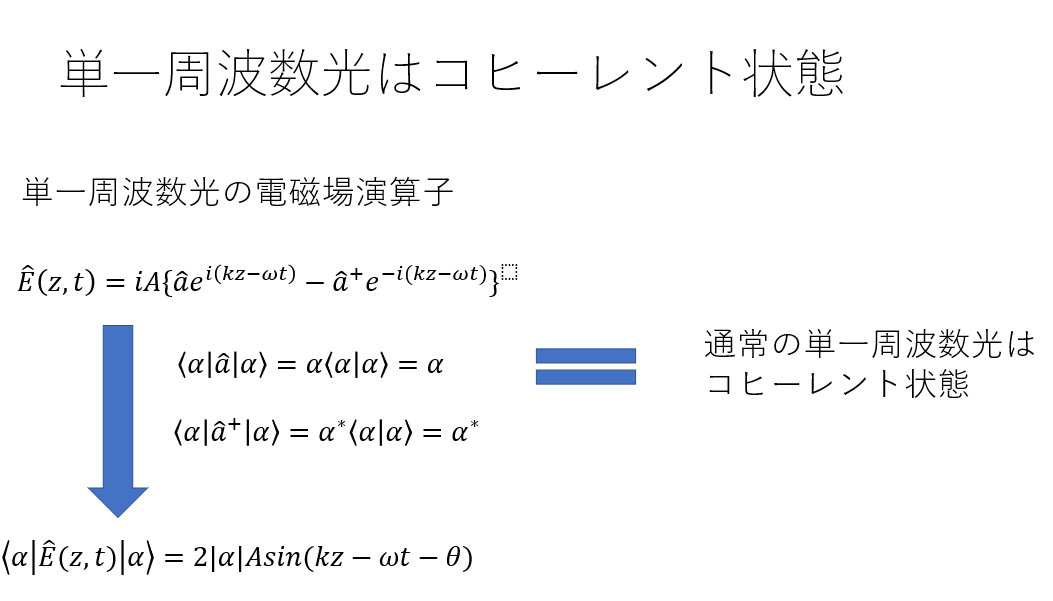
\includegraphics[width=1.0\textwidth]{img/zemi10.png}
        \caption[sample image (png)]{単一周波数光はコヒーレント状態.}
        \label{Fig:1_5_2}
    \end{figure}
    
    \figref{Fig:1_5_2}に示すように通常の単一周波数光はコヒーレント状態としてあらわされる。

\begin{figure}[htbp]
        \centering   
        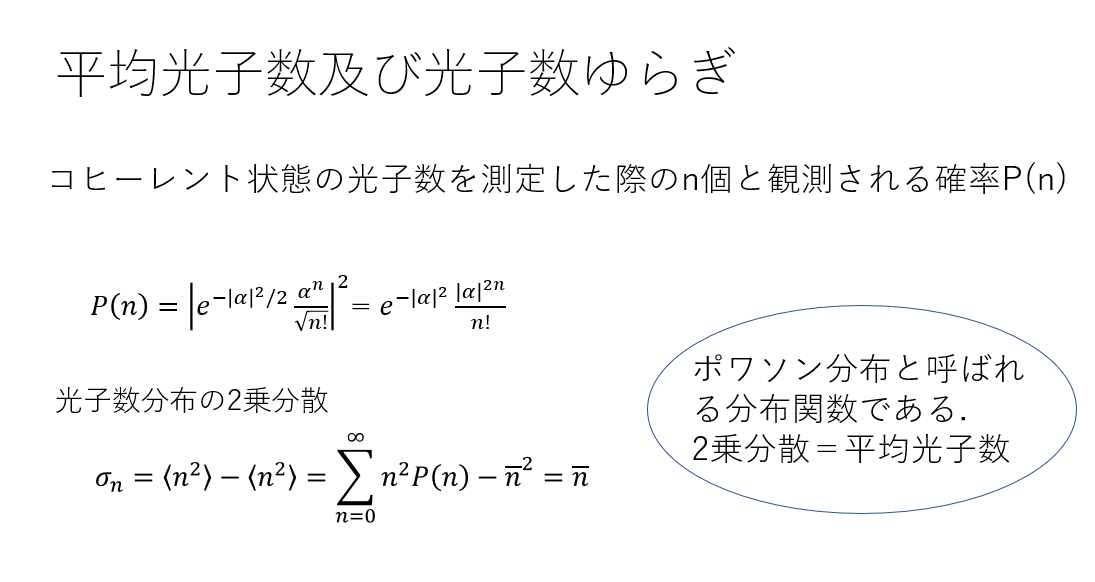
\includegraphics[width=1.0\textwidth]{img/zemi11.png}
        \caption[sample image (png)]{平均光子数及び光子数ゆらぎ.}
        \label{Fig:1_5_3}
    \end{figure}
    
    \figref{Fig:1_5_3}はコヒーレント状態の光子数を測定した際の$n$個と観測される確率$P(n)$について説明している。$P(n)$はポワソン分布と呼ばれる分布関数である。

\begin{figure}[htbp]
        \centering   
        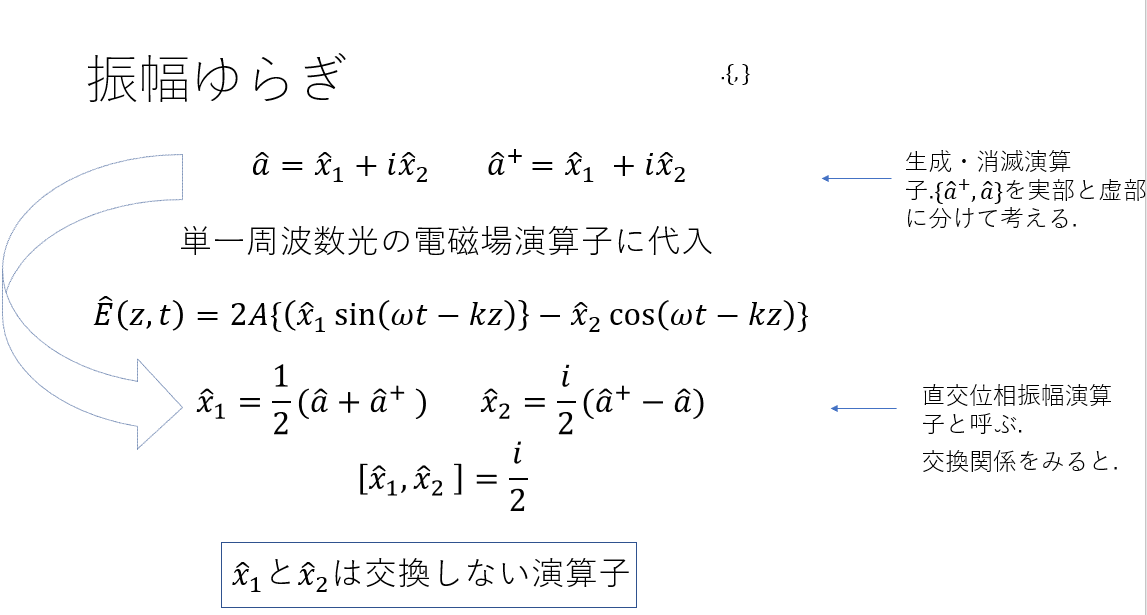
\includegraphics[width=1.0\textwidth]{img/zemi12.png}
        \caption[sample image (png)]{振幅ゆらぎ.}
        \label{Fig:1_5_4}
    \end{figure}

    \figref{Fig:1_5_4}は複素振幅の実部と虚部を表す演算子($\hat{x_1}$),($\hat{x_2}$)の交換関係について説明している。

\begin{figure}[htbp]
        \centering   
        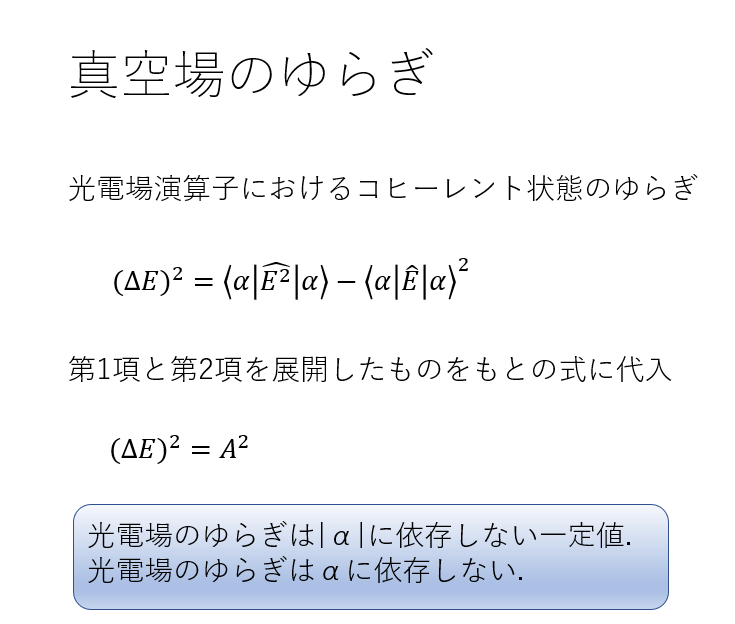
\includegraphics[width=0.8\textwidth]{img/zemi13.png}
        \caption[sample image (png)]{真空場のゆらぎ.}
        \label{Fig:1_5_5}
    \end{figure}
    \figref{Fig:1_5_5}は真空場のゆらぎについて説明しているこのゆらぎは$α$に依存しない.
    
\begin{figure}[htbp]
        \centering   
        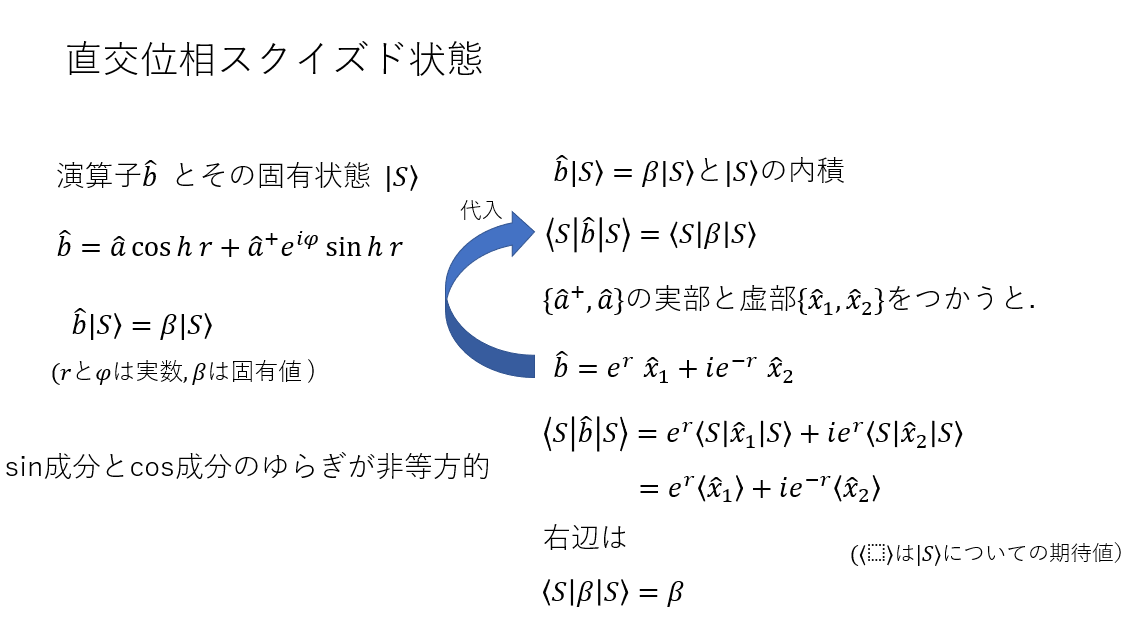
\includegraphics[width=1.0\textwidth]{img/zemi14.png}
        \caption[sample image (png)]{直交スクイズド状態.}
        \label{Fig:1_5_6}
    \end{figure}
    \figref{Fig:1_5_6}はスクイズド状態について説明している。直交位相スクイズド状態は演算子($\hat{b}$)とその固有状態$|{S}\rangle$として与えられる。


\chapter{Y00-量子暗号の信号状態
}
まず、コヒーレント状態について説明する。コヒーレント状態は、複素振幅$\alpha=x+iy$を持つ理想的なレーザー光を表す量子状態である。コヒーレント状態の複素振幅$\alpha$は複素平面上で平均$(x,y)^T$、共分散行列 
$$
\begin{pmatrix}
1/4&0\\
0&1/4
\end{pmatrix}
$$
の正規分布に従って揺らいでいる.\figref{Fig:3_1}は、平均$(x,y)^T$のコヒーレント状態の揺らぎを表している。

\begin{figure}[htbp]
        \centering   
        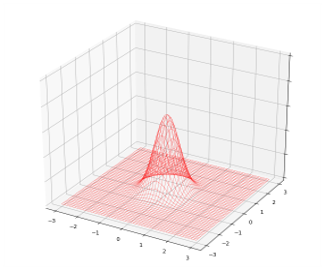
\includegraphics[width=0.7\textwidth]{img/zemi1.png}
        \caption[sample image (png)]{コヒーレント状態のゆらぎ}
        \label{Fig:3_1}
    \end{figure}


Y00-量子暗号の信号状態について説明する。青い丸がコヒーレント状態でこれを使って通信を行う。使用する基底によって0と1に対応する信号状態が異なる。例えば基底1を使って0を送りたいときは0のコヒーレント状態を使い、1を送りたいときは0のコヒーレント状態を使う。正規の受信者と送信者はどの基底を使って通信をしているのかわかる。同じ基底のコヒーレント状態は離れているので盗聴されにくいため、安全性が保証される。$S_{max}$は信号の最大強度を表している.$B$個の規定で通信する場合間隔の個数が$2B-1$個となることから隣接信号間の間隔は$S_{max}/2B-1$になる。このことから基底$k$の信号状態は

$$
\left |\frac{S_{max}}{2B-1}\right\rangle,\left |\frac{S_{max}}{2B-1}(B+k)\right\rangle
$$

\begin{figure}[htbp]
        \centering   
        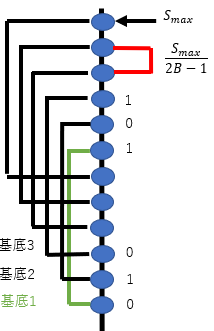
\includegraphics[width=0.5\textwidth]{img/zemi2.png}
        \caption[sample image (png)]{量子暗号の信号状態.}
        \label{Fig:3_2}
    \end{figure}

\chapter{Y00-量子暗号システム}
Y00-量子暗号のシステムについて説明する。送信者と受信者はseedkeyを共有している。まずLFSRによって疑似乱数を発生させる。
このとき、seedkeyが同じであるので発生する乱数も同じとなる。乱数は基底番号を表し、送信者と受信者は同じ基底番号を使うことができる。送信器では送信バイナリデータと基底番号の値に対応する量子状態を送信する。受信器では受け取った量子状態と基底番号を使ってバイナリデータを出力する。次に受信機における処理について説明する。

\begin{figure}[htbp]
        \centering   
        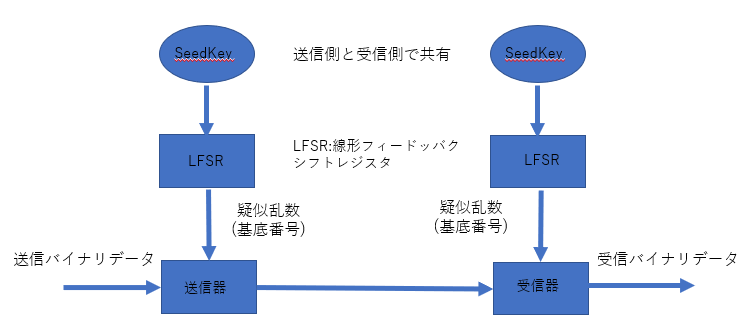
\includegraphics[width=1.0\textwidth]{img/zemi3.png}
        \caption[sample image (png)]{量子暗号システム.}
        \label{fig:4_1}
    \end{figure}



受信器ではまずホモダイン測定を行う。ホモダイン測定はコヒーレント状態の複素振幅$\alpha=x+iy$成分を測定する。\figref{Fig:4_2}は0と1に対応するコヒーレント状態をホモダイン測定した場合の出力の確率分布である。それぞれの分布は分散1/4の正規分布になっている。受信器では、測定値に基づき、しきい値を使って受信したデータが0か1か判断する。

\begin{figure}[htbp]
        \centering   
        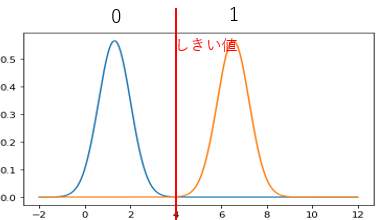
\includegraphics[width=0.7\textwidth]{img/zemi4}
        \caption[sample image (png)]{ホモダイン測定.}
        \label{Fig:4_2}
    \end{figure}
    
\figref{Fig:4_3}は受信機のしきい値処理を説明したものである。2つのコヒーレント状態の値のちょうど真ん中をしきい値とする。基底番号が3の場合それに対応するコヒーレント状態は緑色に示したコヒーレント状態になるが、そのときのしきい値は$\frac{S_{max}}{2B-1}(\frac{B}{2}+k)$となる。また、基底番号が奇数の場合、測定値がしきい値より大きければ1、小さければ0と判定する.基底番号が偶数の場合、測定値がしきい値より大きければ0、小さければ1と判定する。

\begin{figure}[htbp]
        \centering   
        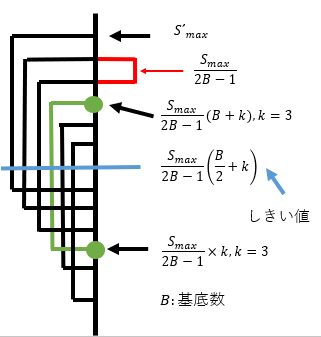
\includegraphics[width=0.5\textwidth]{img/zemi5.png}
        \caption[sample image (png)]{受信機のしきい値処理.}
        \label{Fig:4_3}
    \end{figure}



\chapter{通信路に減衰がある場合}
今回の評価実験では通信路が減衰の影響を受ける場合について考える。
\figref{Fig:5_1}は減衰の影響について表した。
減衰を受けることにより、平均$\mu$は$\sqrt{k}\mu$となる。
また、共分散行列$A$は、$kA+ (1-k)/4 $となる。ここで、$k$は透過率を表す。ただし、コヒーレント状態の場合、共分散行列は減衰によって変化しない。


\begin{figure}[htbp]
        \centering   
        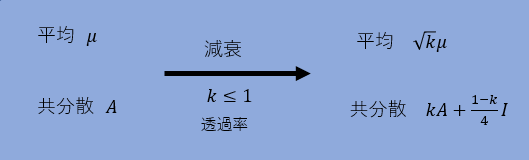
\includegraphics[width=0.8\textwidth]{img/zemi6.png}
        \caption[sample image (png)]{減衰の影響.}
        \label{Fig:5_1}
    \end{figure}





\figref{Fig:5_2}は、今回の評価実験の構成図になる。この通信路が透過率$k$の減衰の影響を受けている。
ここで、送信器の信号の最大強度の設定を$S_{max}$、受信機の信号の最大強度の設定を$S'_{max}$とする。
実験では$S_{max}$と$S´_{max}$が等しい場合と減衰の効果を考慮して$S´_{max}$を決める場合について実験を行った。
また、今回の実験では受信器は乱数を発生させてシミュレートした。
\begin{figure}[H]
        \centering   
        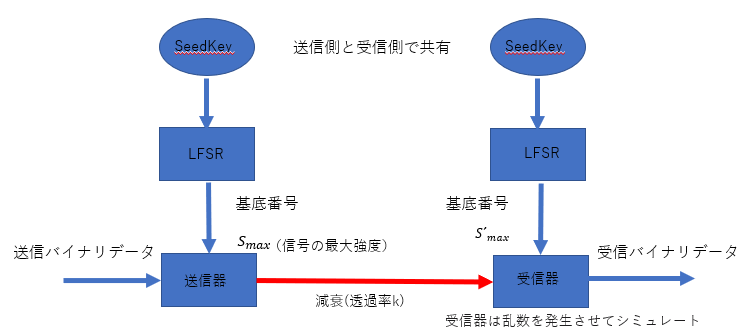
\includegraphics[width=1.0\textwidth]{img/zemi7.png}
        \caption[sample image (png)]{減衰がある場合の正規受信者の誤り率.}
        \label{Fig:5_2}
    \end{figure}


\section{評価実験}
減衰がある場合の正規受信者の誤り率を評価する。以下は送信者側のプログラムである。
\begin{lstlisting}[caption=送信者側のプログラム,label=program1]
import numpy as np
import random

register=np.array([1,0,1,0,1,1,0,0,1,1,1,0,0,0,0,1]) #Seed Keyの設定
#@markdown `基底を決めるのに必要なビット数`
N=8 #@param {type: "number"}

#@markdown `出力される信号の個数`
M=1000 #@param {type: "number"}
BNum=2**N 

#@markdown `信号の最大強度`
#信号の最大強度 (信号の強度は0~S_maxで設定される)
S_max=5 #@param {type: "number"}

S_levels=np.linspace(0,S_max,BNum*2) #使用される信号強度の配列
##--------送受信者共通データ----------##
register=np.array([1,0,1,0,1,1,0,0,1,1,1,0,0,0,0,1]) #Seed Keyの設定

#Driverのためのデータを作成
a=np.zeros(N) #要素数8の配列を0で初期化したものをaに代入
input_Data=np.zeros(M) #送信データは常に0と仮定
#input_Data=[0,1,1,0,1,1,1,0,0,1]
output_qstates=[]

for j in range(M): #データ出力のためのループ
  for i in range(N): #LFSRの出力をNビット分だけ配列aに格納している
    SR=(register[10]+register[12]+register[13]+register[15])%2 
    a[i]=register[15] 
    register=np.roll(register,1) 
    register[0]=SR
    ###
  d=0
  p=1
  ###LFSRからの出力をNビットずつまとめて数値(0~BNum-1)に変換し、Mapperの入力としている
  for i in range(N):
    d+=p*a[i]
    p*=2 
  base_id=int(d)
  index=int(input_Data[j])

#if base_id%2==1:
#    index=(index+1)%2
  index=(index+base_id%2)%2

  output_level=S_levels[base_id+BNum*index] #Driverから出力される信号強度
  q_state=Qstate(output_level) #送信者から出力される量子状態
  output_qstates.append(q_state)
\end{lstlisting}

\begin{lstlisting}[caption=減衰のプログラム,label=program2]
att_rate_total=0.05 #@param {type: "number"}

att_rate=att_rate_total
for j in range(M):
  output_qstates[j].attenuate(att_rate)
\end{lstlisting}

\begin{lstlisting}[caption=受信側のプログラム(最大強度の調整なし),label=program3]

import numpy as np
import random

register=np.array([1,0,1,0,1,1,0,0,1,1,1,0,0,0,0,1]) #Seed Keyの設定

#N=8 


#M=100 
BNum=2**N 


#信号の最大強度 (信号の強度は0~S_maxで設定される)
#S_max*=np.sqrt(att_rate)  #ここを生かして実行してみる
#S_max=10
def getData(q_state,base_id):
  thld=S_max/(2*BNum-1)*(BNum/2+base_id) #base_idからしきい値を決める
  val=q_state.homodyne(thld)
  #print("val:",val)
  #if base_id%2==1:
  #val=(val+1)%2   ##valの値がそのまま出力する際はbase_idが偶数の時のみ,base_idが奇数の時は0と1が反転する
  val=(val+base_id%2)%2
  return val

S_levels=np.linspace(0,S_max,BNum*2) #使用される信号強度の配列
##--------送受信者共通データ----------##
register=np.array([1,0,1,0,1,1,0,0,1,1,1,0,0,0,0,1]) #Seed Keyの設定

#Driverのためのデータを作成
a=np.zeros(N) #要素数8の配列を0で初期化したものをaに代入
input_Data=np.zeros(M) #送信データは常に0と仮定
output_vals=[]

for j in range(M): #データ出力のためのループ
  for i in range(N): #LFSRの出力をNビット分だけ配列aに格納している
    SR=(register[10]+register[12]+register[13]+register[15])%2 
    a[i]=register[15] 
    register=np.roll(register,1) 
    register[0]=SR
    ###
  d=0
  p=1
  ###LFSRからの出力をNビットずつまとめて数値(0~BNum-1)に変換し、Mapperの入力としている
  for i in range(N):
    d+=p*a[i]
    p*=2 
  base_id=int(d)

  output_vals.append(getData(output_qstates[j],base_id)) #出てきた値に対して配列の要素として持つ
  #output_qstates.append(q_state)
  
  #print("-----")
print(np.sum(output_vals)/M)

\end{lstlisting}

\begin{lstlisting}[caption=受信側のプログラム(最大強度の調整あり),label=program4]


import numpy as np
import random

register=np.array([1,0,1,0,1,1,0,0,1,1,1,0,0,0,0,1]) #Seed Keyの設定

#N=8 


#M=100 
BNum=2**N 


#信号の最大強度 (信号の強度は0~S_maxで設定される)
S_max*=np.sqrt(att_rate)  #ここを生かして実行してみる
#S_max=10
def getData(q_state,base_id):
  thld=S_max/(2*BNum-1)*(BNum/2+base_id) #base_idからしきい値を決める
  val=q_state.homodyne(thld)
  #print("val:",val)
  #if base_id%2==1:
  #val=(val+1)%2   ##valの値がそのまま出力する際はbase_idが偶数の時のみ,base_idが奇数の時は0と1が反転する
  val=(val+base_id%2)%2
  return val

S_levels=np.linspace(0,S_max,BNum*2) #使用される信号強度の配列
##--------送受信者共通データ----------##
register=np.array([1,0,1,0,1,1,0,0,1,1,1,0,0,0,0,1]) #Seed Keyの設定

#Driverのためのデータを作成
a=np.zeros(N) #要素数8の配列を0で初期化したものをaに代入
input_Data=np.zeros(M) #送信データは常に0と仮定
output_vals=[]

for j in range(M): #データ出力のためのループ
  for i in range(N): #LFSRの出力をNビット分だけ配列aに格納している
    SR=(register[10]+register[12]+register[13]+register[15])%2 
    a[i]=register[15] 
    register=np.roll(register,1) 
    register[0]=SR
    ###
  d=0
  p=1
  ###LFSRからの出力をNビットずつまとめて数値(0~BNum-1)に変換し、Mapperの入力としている
  for i in range(N):
    d+=p*a[i]
    p*=2 
  base_id=int(d)

  output_vals.append(getData(output_qstates[j],base_id)) #出てきた値に対して配列の要素として持つ
  #output_qstates.append(q_state)
  
  #print("-----")
print(np.sum(output_vals)/M)

\end{lstlisting}



\figref{Fig:5_4}は信号の最大強度が5、基底数が256、送信データ数が1000個の場合に透過率と正規受信者の誤り率の関係を表したものである。また、縦軸は誤り率、横軸は透過率で、透過率を0〜0.05づつ1.0まで上げた際の変化をまとめた。グラフからわかる通り、信号の最大強度を調整することで、0.05〜0.6の間で誤り率を大幅に減らすことができることがわかる。また透過率が0.8~1.0の範囲では信号の最大強度を調整しなくても信号の誤り率が低くなることがわかる。

\begin{figure}[htbp]
        \centering   
        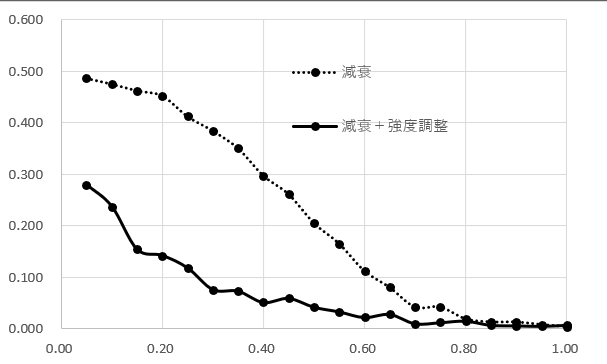
\includegraphics[width=1\textwidth]{img/zemi16.png}
        \caption[sample image (png)]{透過率と正規受信者の誤り率の関係.}
        \label{Fig:5_4}
    \end{figure}
\chapter{増幅器の効果}
減衰通信路に増幅器を設置する効果について評価を行う。
増幅器の設置位置としては減衰通信路のちょうど真ん中に設置する場合と、受信器の直前に設置する場合について考える。
以下は増幅器を減衰通信路のちょうど真ん中に設置する場合の減衰+増幅+減衰のプログラムである。
\begin{lstlisting}[caption=減衰+増幅+減衰のプログラム,label=program6]

att_rate_total=0.9
att_rate=np.sqrt(att_rate_total)
gain=1/att_rate
for j in range(M):
  output_qstates[j].attenuate(att_rate)
  output_qstates[j].amplificate(gain)
  output_qstates[j].attenuate(att_rate)

\end{lstlisting}

また、以下は更に前置増幅器も設置する場合の、減衰+増幅+減衰+
前置増幅のプログラムである。

\begin{lstlisting}[caption=減衰+増幅+減衰+前置増幅のプログラム,label=program7]

att_rate_total=0.9
att_rate=np.sqrt(att_rate_total)
gain=1/att_rate
for j in range(M):
  output_qstates[j].attenuate(att_rate)
  output_qstates[j].amplificate(gain)
  output_qstates[j].attenuate(att_rate)
  output_qstates[j].amplificate(gain)

\end{lstlisting}


次に、増幅器を減衰通信路の中間位置においた場合の評価を行う。また、前置増幅を行った場合と前置増幅を行わず強度調整を行った場合の比較も合わせて行うことにする。\figref{Fig:5_5}は信号の最大強度が5、基底数が256、送信データ数が1000個の場合に透過率と正規受信者の誤り率の関係を表したものである。

本実験では、信号が受信される直前に増幅をさせる(前置増幅)。増幅のみを行った場合に比べると誤り率は低く見られたが増幅と信号強度の調整を行った場合に比べると誤り率は少し高くなっている。

\begin{figure}[htbp]
        \centering   
        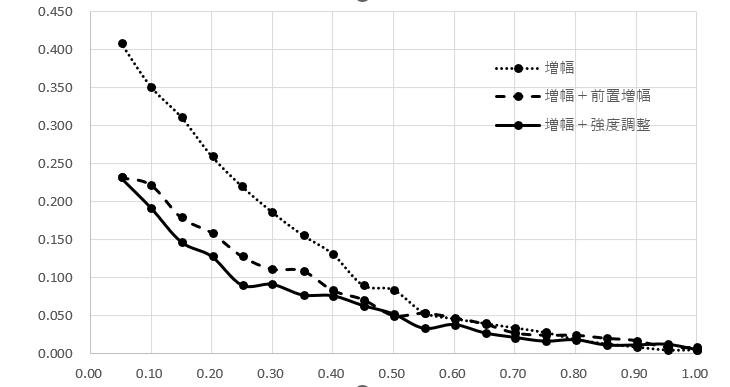
\includegraphics[width=1\textwidth]{img/zemi1-2.png}
        \caption[sample image (png)]{前置増幅と誤り率の関係.}
        \label{Fig:5_5}
    \end{figure}
\chapter{結論}
 本研究ではY00-量子暗号のシミュレーションシステムを用いて正規受信者の誤り率の評価を行った。また、信号強度の調整を行った場合についてもまとめた。誤り率がもっとも低くなったのが強度調整をし、減衰の影響を受けたものである。反して、増幅と前置増幅を行った場合では増幅のみを行ったときに比べ誤り率が少し上がってしまった。
%\chapter*{謝辞}
\addcontentsline{toc}{chapter}{謝辞}

本研究は, 東京大学 大学院 情報理工学系研究科 知能機械情報学専攻 your professor 教授のご指導のもとで行われました.
%\bibliographystyle{bib/IEEEtransBST/IEEEtran}
\bibliography{bib/style,bib/liter}

\renewcommand{\prechaptername}{付録}
\renewcommand{\postchaptername}{}
\renewcommand{\thechapter}{\Alph{chapter}}
\setcounter{chapter}{0}

\chapter{量子状態のクラスのプログラム}
\begin{lstlisting}[caption=量子状態のクラス,label=Qstate]
# -*- coding: utf-8 -*-
import cmath
import math
import numpy
from scipy.stats import norm
import numpy as np
import numpy.linalg as LA
import matplotlib.pyplot as plt

#振幅値 
A = 1.0
#行列Jを指定
J = np.array([[0, 1] , [-1, 0]])
#単位行列Iを指定
Id = np.array([[1.0, 0] , [0 , 1.0]])  

class Qstate:
    """量子ガウス状態を表すクラス"""
    def __init__(self, c_amplitude = A + 0j ):
        """初期値の設定を追加 (sohma Aug 12 2018)"""
        # 複素振幅値
        self.alpha = c_amplitude

        # コヒーレント状態の正規分布の広がり(共分散行列)を表す        
        self.a = np.array([[0.25 , 0] , [0 , 0.25]])

        # 正規受信者の確率        
        self.Pr = 0.0
        
        
    def attenuate(self, att_rate):
        """減衰する
           aの値(共分散)と平均が変換される"""
        #減衰後の複素振幅を計算
        self.alpha = self.alpha* math.sqrt(att_rate)
        #減衰後の共分散行列を計算
        self.a = (att_rate * self.a) + ((1.0-att_rate) * Id / 4.0)

    def amplificate(self,gain):
        """増幅する
           aの値(共分散)と平均が変換される"""
        #増幅後の複素振幅を計算
        self.alpha =  self.alpha* math.sqrt(gain)
        #増幅後の共分散行列を計算
        self.a = (gain * self.a) + ((gain-1.0) * Id / 4.0)


    def measure_homodyne(self, theta_val):
        """ホモダイン測定を行う"""     
        # 量子状態を元の位置まで回転させる
        rev_rot =  cmath.rect(1.0, theta_val)
        beta =  self.alpha * rev_rot
        U = np.array([[math.cos(theta_val) , -math.sin(theta_val)] , [math.sin(theta_val) , math.cos(theta_val)]])
        b = np.dot(U.T , np.dot(self.a , U))
        
        # 共分散行列 b の x軸方向の標準偏差
        dev_x = math.sqrt(b[0, 0])
        
        # 0が出力される確率(測定値が正になる確率)       
        self.Pr =  norm.sf(x = 0.0 , loc = beta.real ,scale = dev_x )
        return self.Pr
    
    def homodyne_measurement(self):
        dev_x=math.sqrt(self.a[0,0])
        res = np.random.normal(loc=np.real(self.alpha), scale = dev_x)
        return res

    def plot_distribution(self,ax,max_x,max_y,min_x,min_y,c_name="blue"):  
      x = np.arange(min_x, max_x, 0.01) # x点として[min_x, max_y]まで0.01刻みでサンプル
      y = np.arange(min_y, max_y, 0.01)  # y点として[min_x, max_y]まで0.01刻みでサンプル
      x, y = np.meshgrid(x, y)  # 上述のサンプリング点(x,y)を使ったメッシュ生成
      dev_x=math.sqrt(self.a[0,0])   #共分散行列を表す属性a[0,0]の平方根をdev_xに代入
      dev_y=math.sqrt(self.a[1,1])   #共分散行列を表す属性a[1,1]の平方根をdev_yに代入
      z = norm.pdf(x,self.alpha.real,dev_x)*norm.pdf(y,self.alpha.imag,dev_y)
      ax.set_zlim(0.0,1.0)
      ax.plot_wireframe(x, y, z, color=c_name,linewidth=0.3) # ワイヤーフレームのプロット。color,linewidthは曲面のメッシュの線の色と太さをそれぞれ表す。

      ax.tick_params(labelbottom="off",bottom="off") # x軸の削除
      ax.tick_params(labelleft="off",left="off") # y軸の削除
      #ax.set_xticklabels([]) 
      #ax.set_yticklabels([])
      ax.set_zticklabels([])

    def homodyne(self,thld):#arrがthld(しきい値)より大きければ1,小さければ0を出力する
      arr=np.random.normal(self.alpha.real,np.sqrt(self.a[0][0]),1) #平均self.alpha.real,標準偏差np.sqrt(self.a[0][0]),乱数を1個出力する正規分布をarrに代入
      #print("arr:",arr,"thld:",thld)
      if arr>thld:
        return 1
      else:
        return 0
         #1か0を出力する
\end{lstlisting}



\renewcommand{\prechaptername}{付録}
\renewcommand{\postchaptername}{}
\renewcommand{\thechapter}{\Alph{chapter}}

\chapter{光の量子状態について}


\begin{figure}[htbp]
        \centering   
        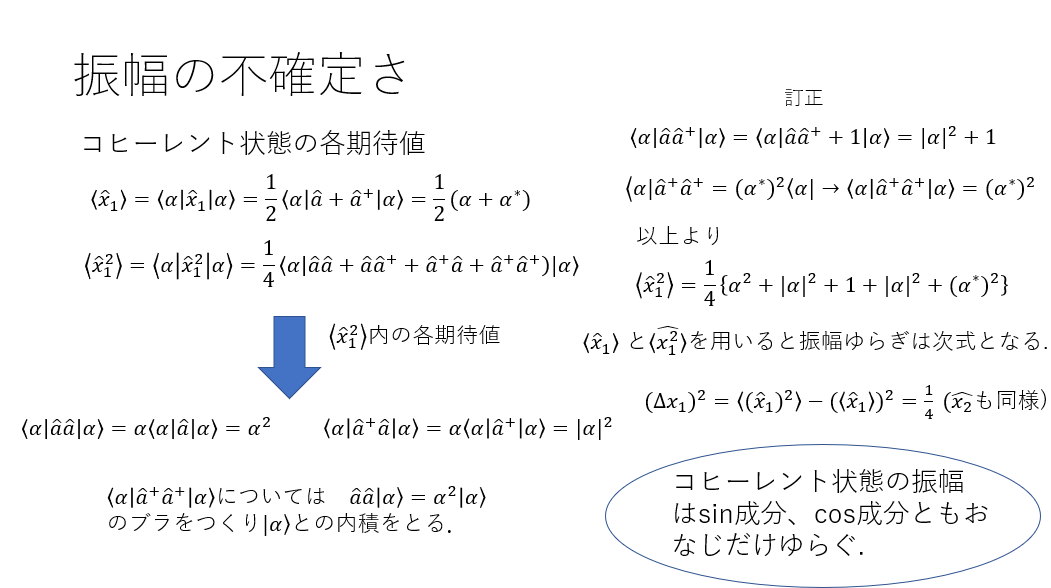
\includegraphics[width=0.8\textwidth]{img/zemi20.png}
        \caption[sample image (png)]{振幅の不確定さ.}
        \label{Fig:1_7_5}
    \end{figure}
    
\begin{figure}[htbp]
        \centering   
        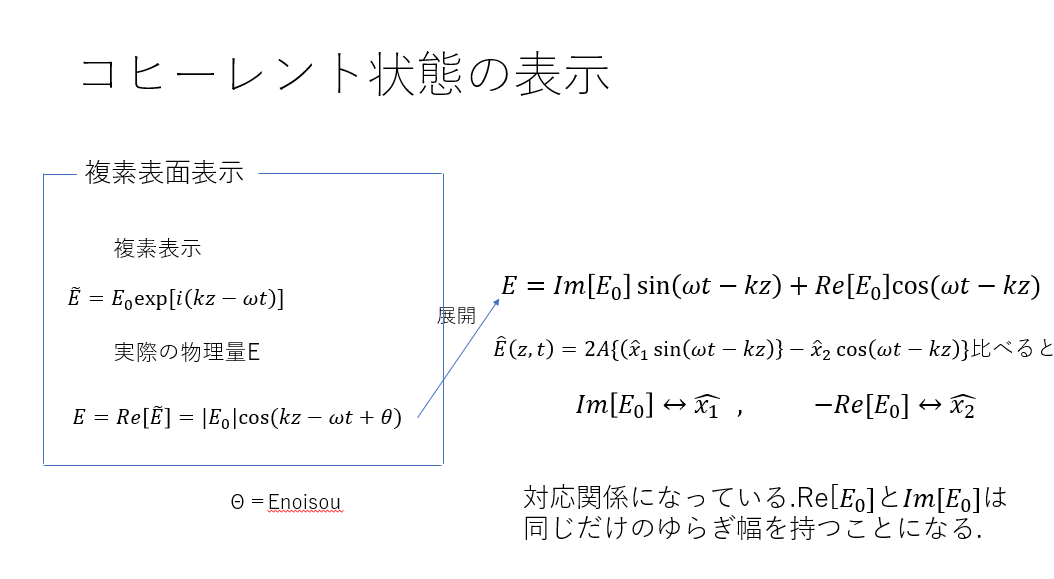
\includegraphics[width=0.8\textwidth]{img/zemi21.png}
        \caption[sample image (png)]{コヒーレント状態の表示.}
        \label{Fig:1_7_6}
    \end{figure}
    
\begin{figure}[htbp]
        \centering   
        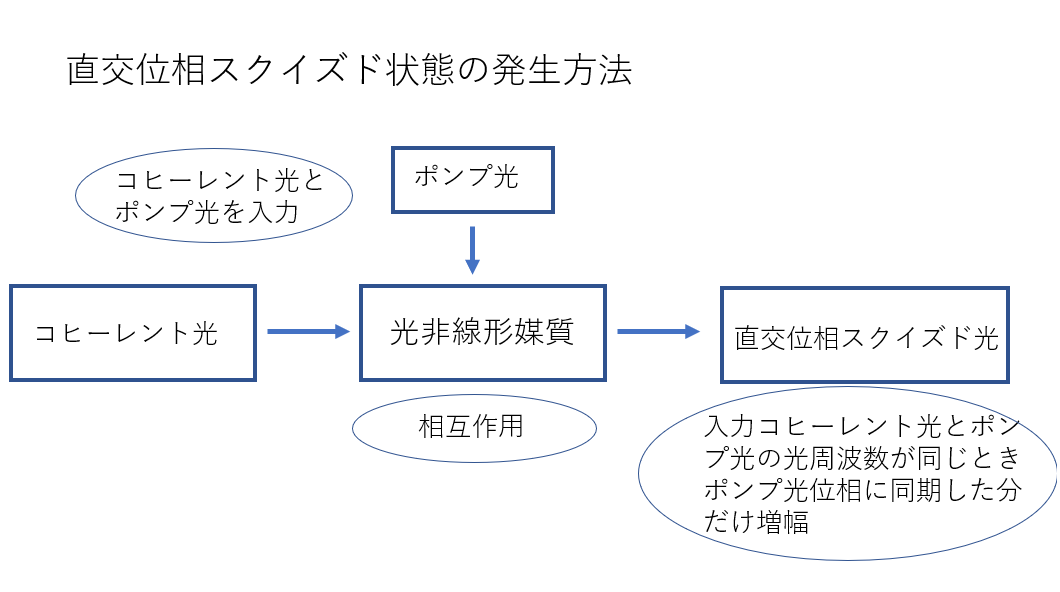
\includegraphics[width=0.8\textwidth]{img/zemi22.png}
        \caption[sample image (png)]{直交位相スクイズド状態の発生方法.}
        \label{Fig:1_7_7}
    \end{figure}

% 後書き
\backmatter
\appendix

\printindex
\end{document}